\documentclass[10pt, aspectratio = 169]{beamer}
\usetheme{Soton}
\usecolortheme{default}
%\usepackage{pifont}
%\usepackage{enumitem}
\usepackage{graphicx} % Allows including images
\usepackage{animate}
\usepackage{caption}
\usepackage{booktabs}
\usepackage{xcolor} 
\usepackage{mathtools}
\usepackage{environ}
\usepackage{multirow}
%\usepackage[textfont={scriptsize,it}]{caption}
\usepackage{listings}
\usepackage{minted}
%\usepackage{subcaption}
\usepackage{braket}% Allows the use of \toprule, \midrule and \bottomrule in tables
%\usepackage[capbesideposition=right]{floatrow}
\setbeamerfont{footnote}{size=\tiny}
\usepackage[absolute,overlay]{textpos}
\usepackage{tikz}
\usetikzlibrary{backgrounds}

\pgfdeclarelayer{background}
\pgfdeclarelayer{foreground}
\pgfsetlayers{background,main,foreground}

\title{Omnifold uncertainties} % The short title appears at the bottom of every slide, the full title is only on the title page
\subtitle{How statistical uncertainties propagate through unbinned unfolding}

\author{Tanmay Pani }
%\supervisors[Supervised by]{Prof. Sevil Salur}
\institute{Rutgers University}

\date{\today} % Date, can be changed to a custom date
\setTitleLogoLeft{Rutgers}
\setTitleLogoRight{STAR-logo}

\setLogo{STAR-logo}


\begin{document}
	
	\begin{frame}
		\titlepage
	\end{frame}
	
	\begin{frame}
		\frametitle{Multi-Layer Perceptron (MLP) - Toy Example}
			


		\begin{columns}
			\begin{column}{0.5\paperwidth}
				\only<1>{
					\begin{figure}
						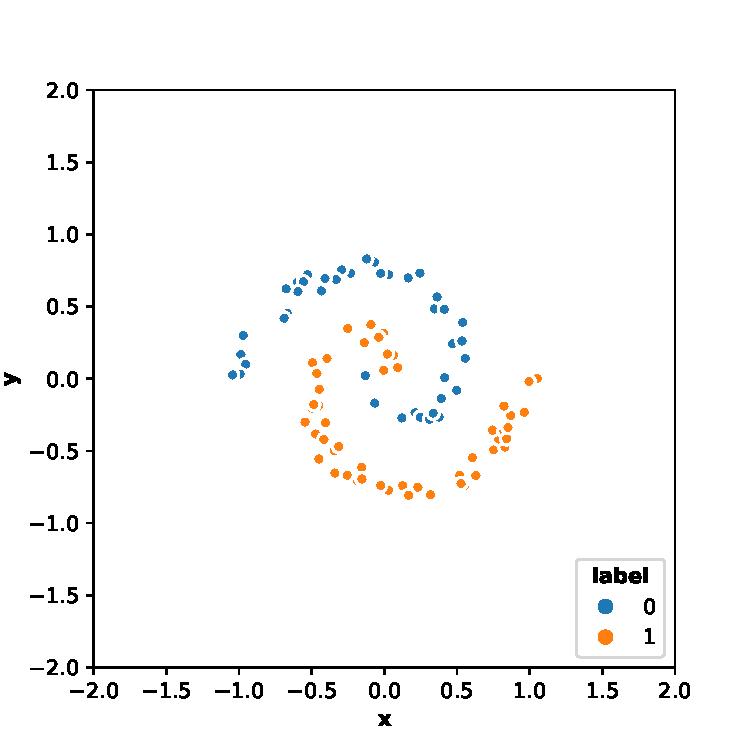
\includegraphics[width=0.8\linewidth]{toy-example/data}
					\end{figure}
				}
				\only<2>{
						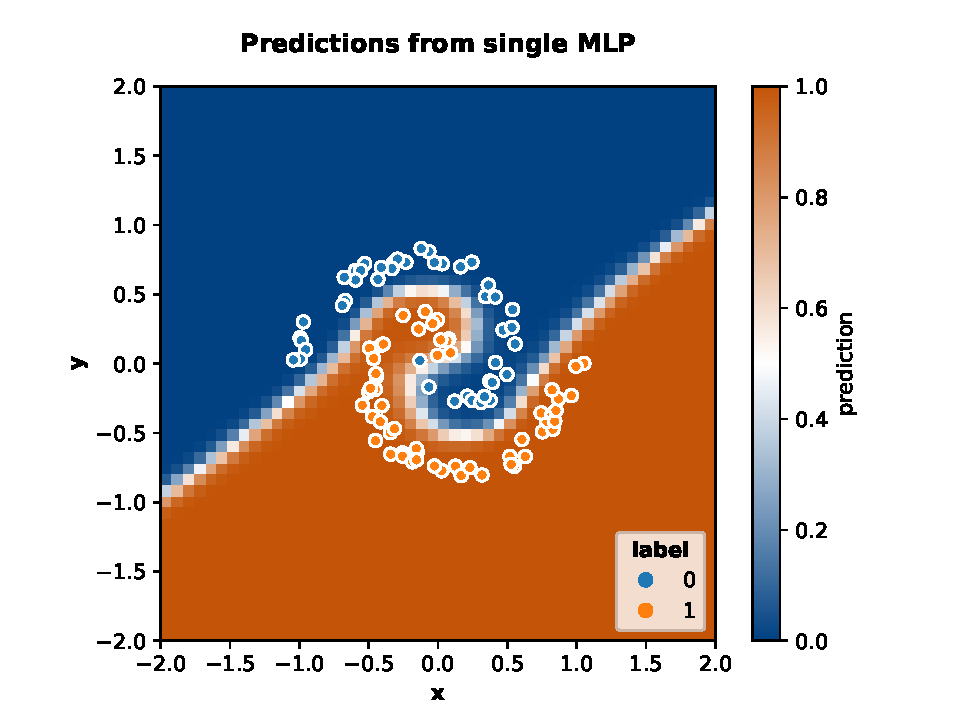
\includegraphics[width=\linewidth]{toy-example/predictions_single}				
				}
				\only<3>{
					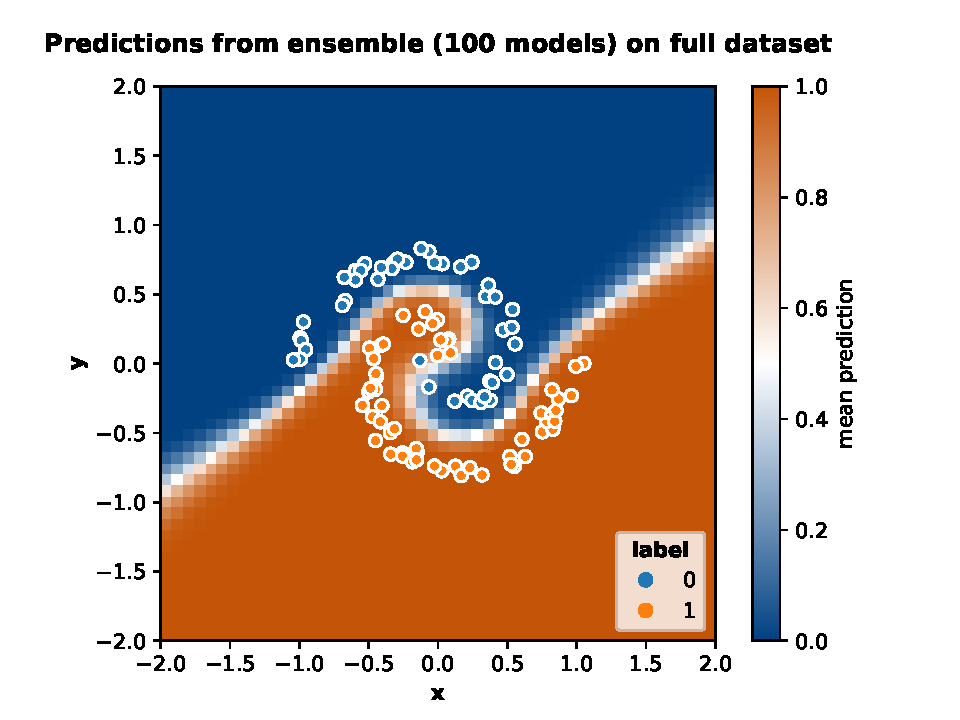
\includegraphics[width=\linewidth]{toy-example/predictions_parallel_no_bootstrap}				
				}
				\only<4>{
					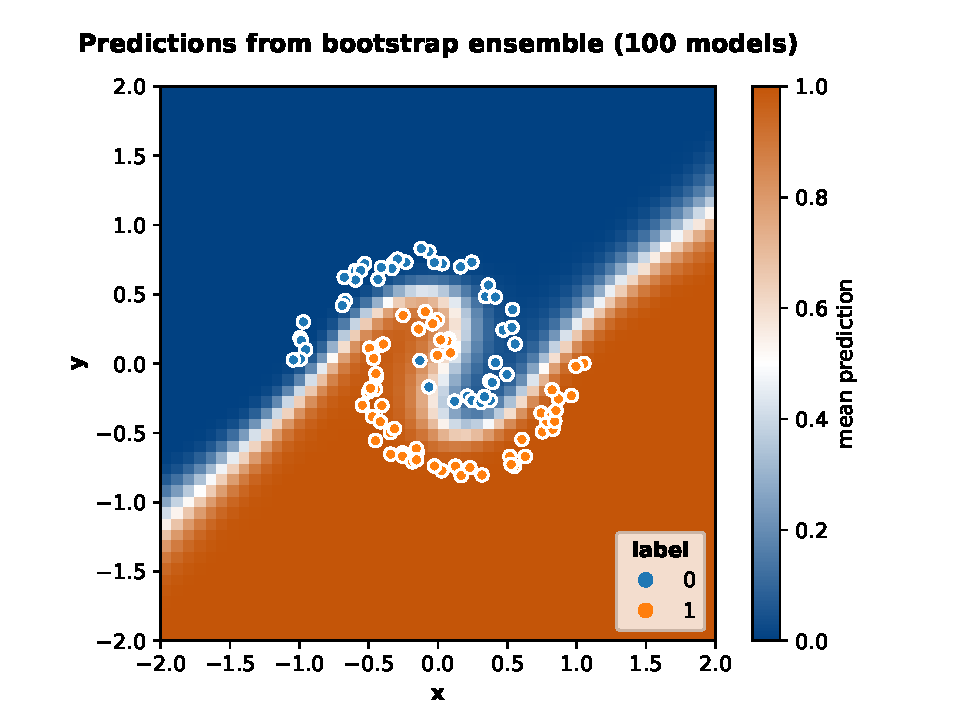
\includegraphics[width=\linewidth]{toy-example/predictions_parallel.pdf}				
				}
			\end{column}
			\begin{column}{0.45\paperwidth}
					\only<1>  {\textbf{Dataset:} 100 samples from 2 gaussian-smeared spirals, 
						``0" (upper spiral / blue points ) and ``1" (lower spiral / orange points) \\
						\textbf{Task:} classify the blue and orange points
					}

				\only<2>{
					 \textbf{Attempt 1:} A single Multi-Layer Perceptron (MLP)
					\begin{figure}
					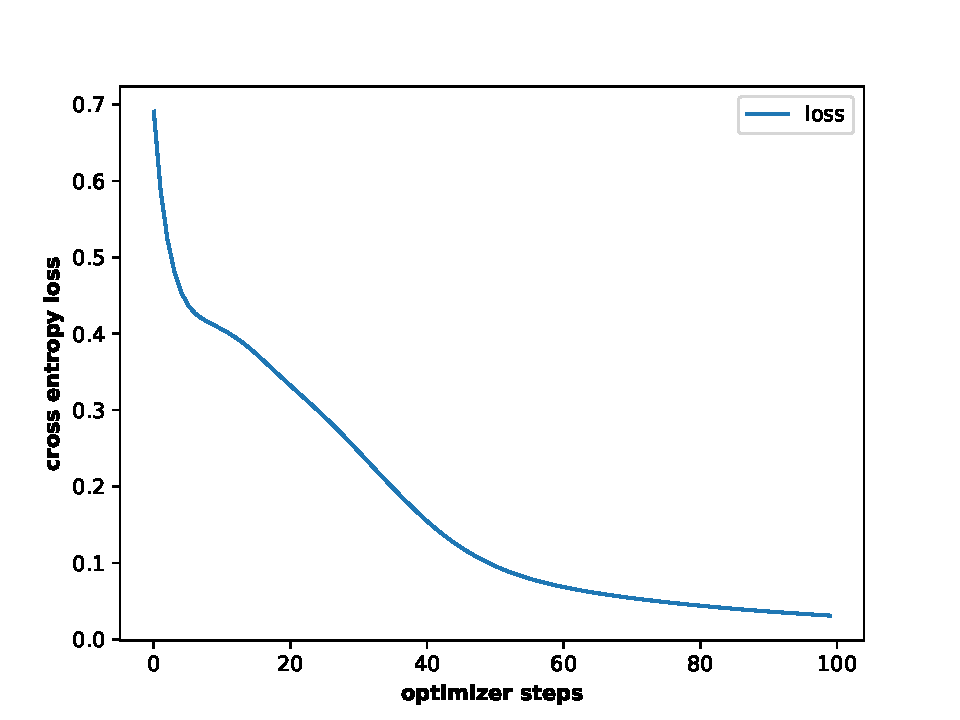
\includegraphics[width=\linewidth]{toy-example/loss_single_model}
				\end{figure}
				}
				\only<3>{
					 \textbf{Attempt 2:} 100 MLPs, each initialized differently, but sees the whole dataset 
					\begin{figure}
						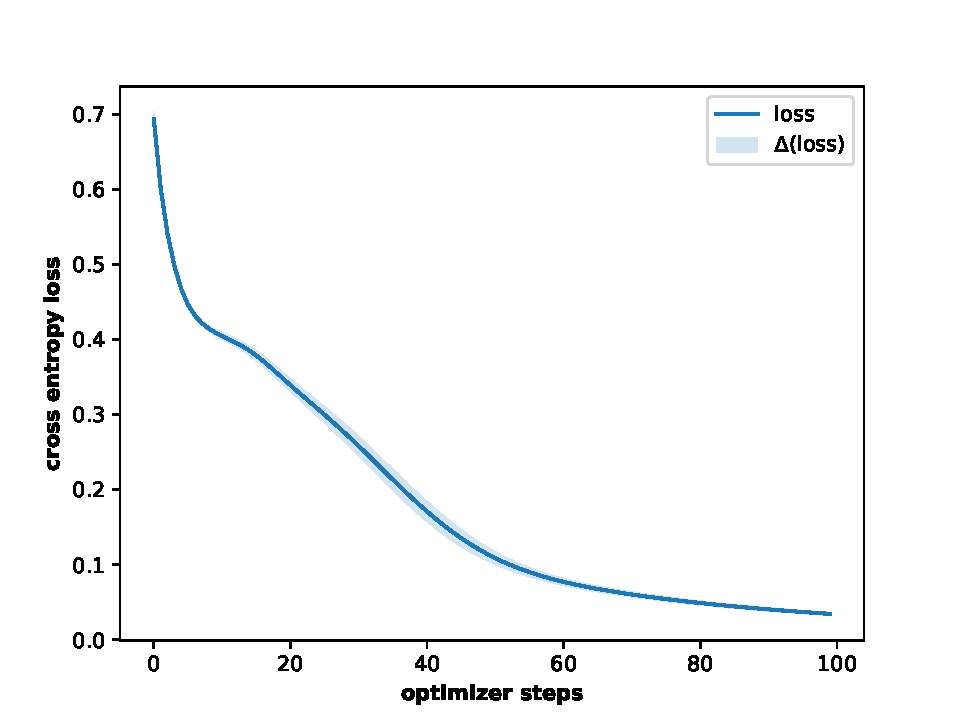
\includegraphics[width=\linewidth]{toy-example/loss_parallel_no_bootstrap.pdf}
					\end{figure}
				}
				
				\only<4>{
					\textbf{Attempt 3:} 100 MLPs, each sees different bootstrap sampling of the dataset 
					\begin{figure}
						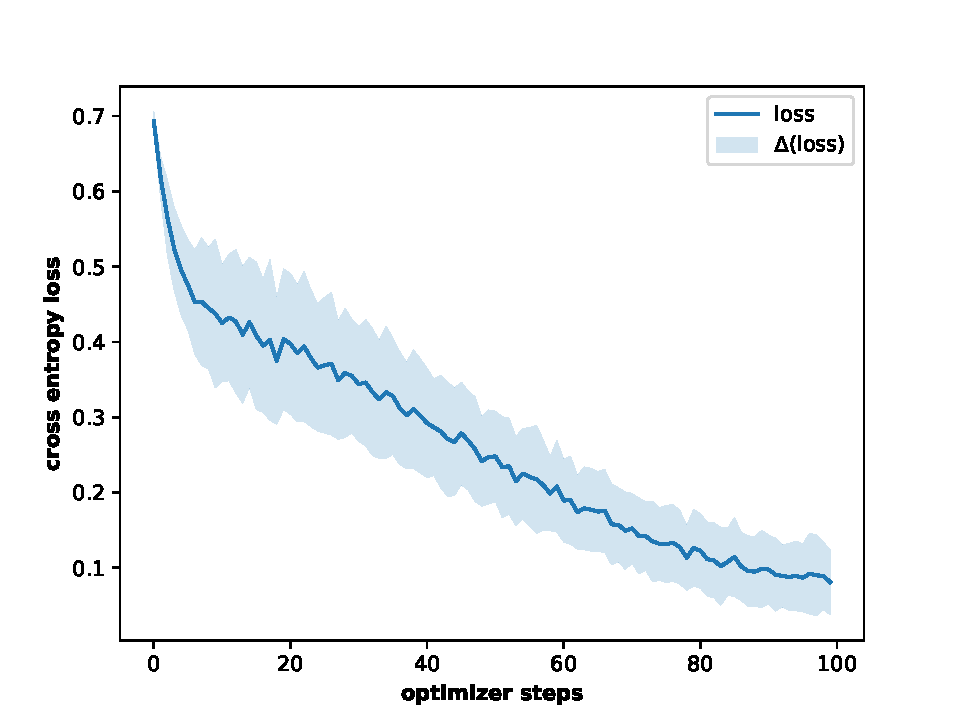
\includegraphics[width=\linewidth]{toy-example/loss_parallel}
					\end{figure}
				}
			\end{column}
		\end{columns}
%		\only<2>{
%		\begin{tikzpicture}[remember picture, overlay]
%				\tikzset{alertbox/.style={
%						fill=red!20, % Light red background
%						draw=red!70!black, % Darker red border
%						thick, % Thicker border
%						rounded corners, % Rounded corners for a softer look
%						text width=0.8\textwidth, % Control text width within the node
%						align=left, % Align text to the left
%						inner sep=1em % Padding inside the box
%					}
%				}
%				
%				% Create the alert box node
%				\node[alertbox] (alert) at (0.45\paperwidth,0.55\paperheight) {
%					\textbf{Important Alert!} \\
%					This is an important message highlighted using a custom TikZ node.
%					Pay close attention to this information.
%				};
%				
%		\end{tikzpicture}
%	}
		
	\end{frame}
	
	\begin{frame}
		\frametitle{Omnifold : Basics}
		\begin{columns}
			\begin{column}{0.5\paperwidth}
				\begin{figure}
					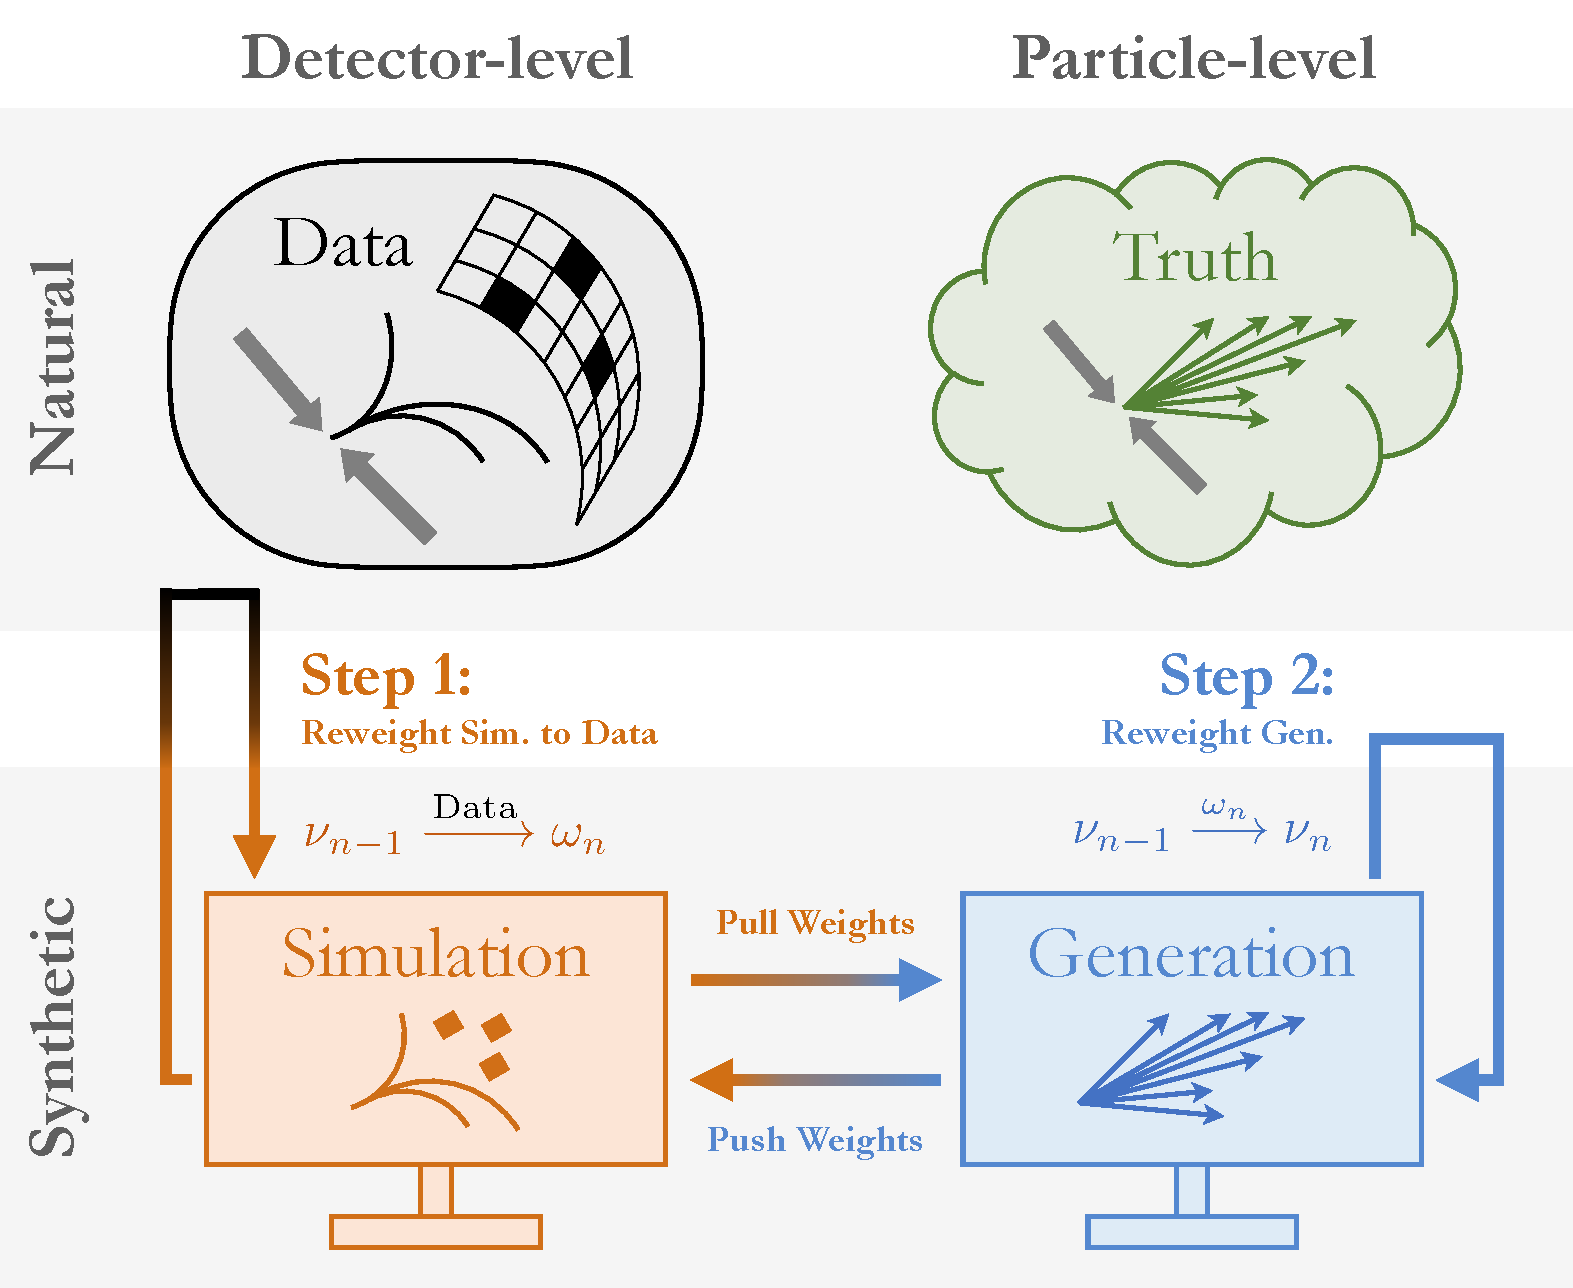
\includegraphics[width=\linewidth]{omnifold_schematic.pdf}
				\end{figure}
			\end{column}
			\begin{column}{0.45\paperwidth}
				\begin{itemize}
					\item<1-> Iterative unfolding using unbinned data
					\item<2-> Steps 1 and  2 each uses MLP classifier to calculate per-sample conditional probabilities
					\item<3->  Step 1 reweights reco to data and Step 2 propagates them to the gen
				\end{itemize}
			\end{column}
		\end{columns}
	\end{frame}
	
		\begin{frame}
		\frametitle{Generalized angularities}
		
		\begin{align}
			\lambda_\beta^\kappa=\sum_{\mathrm{const} \in \mathrm{jet}}\overbrace{ \left(\frac{p_{\rm T, const}}{p_ {\rm T,  jet}}\right)^\kappa}^{\text{\color{red} soft/hard radiation}} \times \overbrace{r(\mathrm{const, jet})^\beta}^{\text{\color{red}collinearity sensitive}} \notag 
		\end{align}
		
		\small$r(\mathrm{const, jet}) = \sqrt{(\eta_{\rm jet}-\eta_{\rm const})^2 + (\phi_{\rm jet}-\phi_{\rm const})^2} $
		
		\begin{itemize}
			%\item Jet substructure observables extracted from angular dependence  of intra-jet energy distribution
			\item \textbf{LHA angularity} $\lambda_{0.5}^1 =\frac{\sum_{\rm trk\in jet} p_{\rm T, trk} \sqrt{\Delta R}}{p_{\rm T, jet}} $,
			\item \textbf{Jet girth: } $\mathbf{g} = \lambda_1^1 =\frac{\sum_{\rm trk\in jet} p_{\rm T, trk} \Delta R}{p_{\rm T, jet}}$, measure of jet broadening
			\item \textbf{Thrust} $\lambda_2^1 =\frac{\sum_{\rm trk\in jet} p_{\rm T, trk} \Delta R^2}{p_{\rm T, jet}} $, related to jet mass
			\item \textbf{Momentum dispersion : $p_T^D = \lambda^2_0$} 
			% \footnote{$\langle y\rangle_x$ refers to average of $y$ over all values of $x$; $\langle y\rangle_x = \frac{\int_x y(x) dx}{\int_x dx}$}
			
			\item Done for both inclusive jets and hard-core component of the inclusive jets
			\item Hard-core component calculated by vector summing constituents with $p_T > 2.0$ GeV/c
		\end{itemize}
	\end{frame}
	
	\begin{frame}
		\frametitle{Dataset and Simulations}
		\begin{itemize}
			\item<1-> \textbf{System:} $p$+$p$ (2012) @ $\sqrt{s_{\rm NN}} = 200$GeV 
			\item<2-> \textbf{High Tower (HT) triggered }events ($\exists$ tower with $E_{\rm tower} \geqslant 4$ GeV) to enhance jet signal
			%\item $|Z_{\rm vertex, event}| < 30$ cm
			\item<3-> \textbf{Embedding simulation: } 	
			\item<4-> \textcolor{red}{GEN: }PYTHIA-6 Perugia-STAR dijet events (\href{https://drupal.star.bnl.gov/STAR/theses/phd-79}{J. K. Adkins, PhD thesis (Kentucky U., 2015)})%\footnote{Phys. Rev. D 82, 074018} 
			\item<4-> \textcolor{blue}{RECO: }PYTHIA-6 Perugia-STAR + GEANT3 +  STAR $p$+$p$ Run12 ZeroBias (2023 version)
				\item<5->  Bootstraped ensembles consists of 10 parallel models and each model sees a bootstrap subsample consisting of 500000 data jets and 500000 reco-jets
			\item<6-> Each model runs for 10 unfolding iterations
		\end{itemize}
	\end{frame}
	
	
	\begin{frame}
		\frametitle{Bootstrapped Omnifolding :  Mean Model Prediction}
			\animategraphics[autoplay,loop,width=\linewidth]{1}{unfolded_hist/wts_iteration_}{0}{5}
	\end{frame}
	
	\begin{frame}
		\frametitle{Bootstrapped Omnifolding :  Unfolded Histograms}
		\begin{figure}
			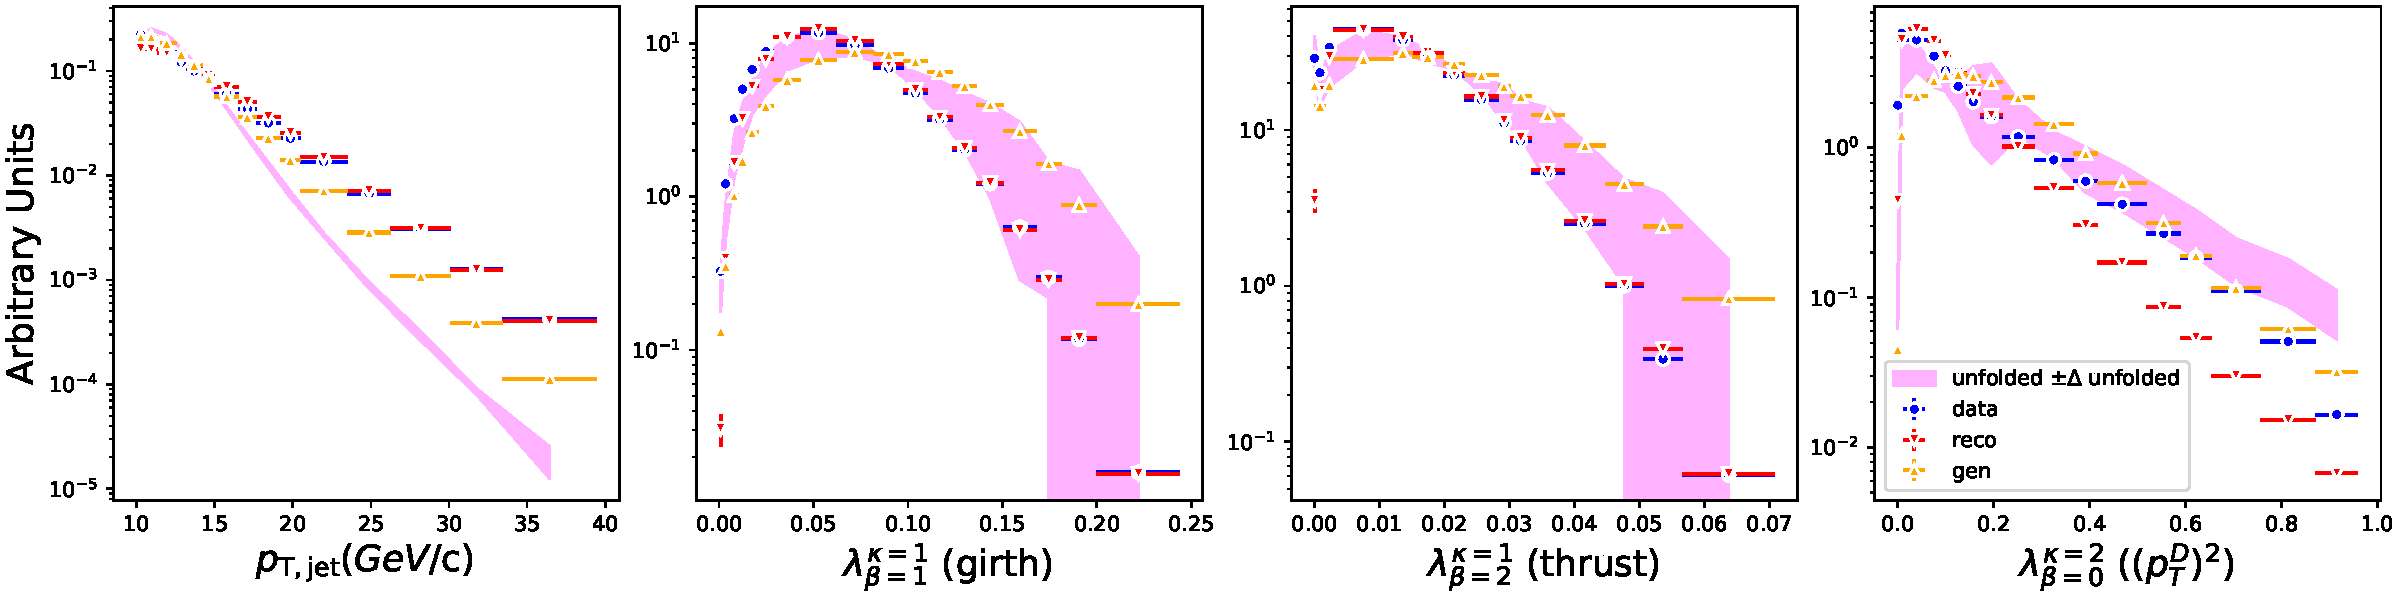
\includegraphics[width=\linewidth]{unfolded_hist/iteration_4.pdf}
									%\caption{Iteration 3}
		\end{figure}
		%		}
%		\only<1>{
%			\begin{figure}
%				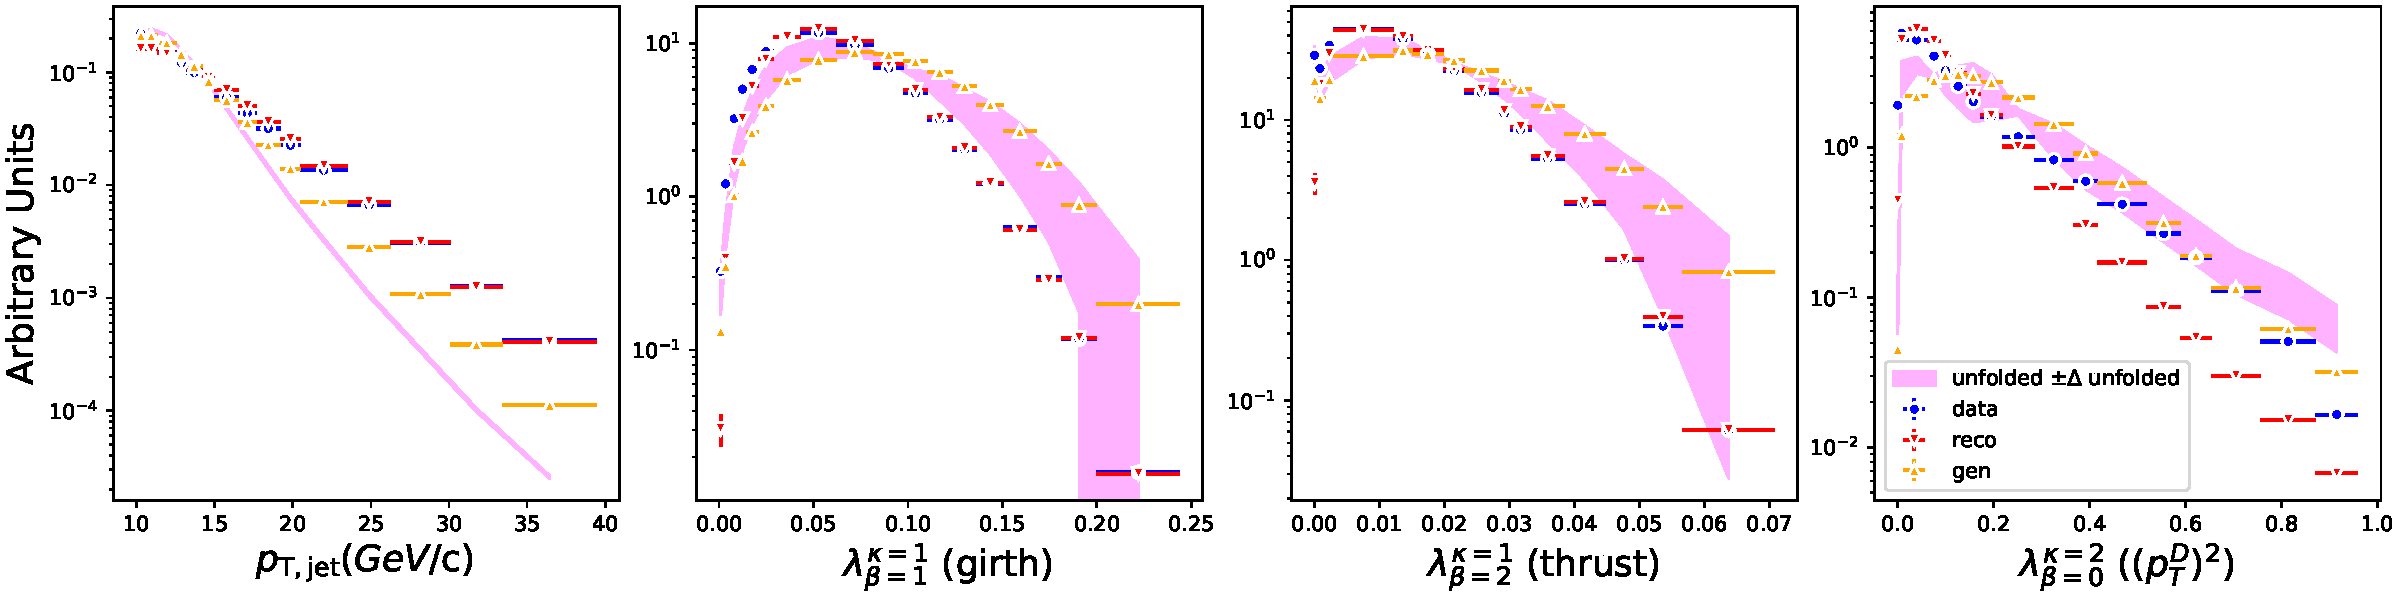
\includegraphics[width=\linewidth]{unfolded_hist/iteration_3.pdf}
%							\caption{Iteration 3}
%			\end{figure}
%		}
%		\only<2>{
%		\begin{figure}
%			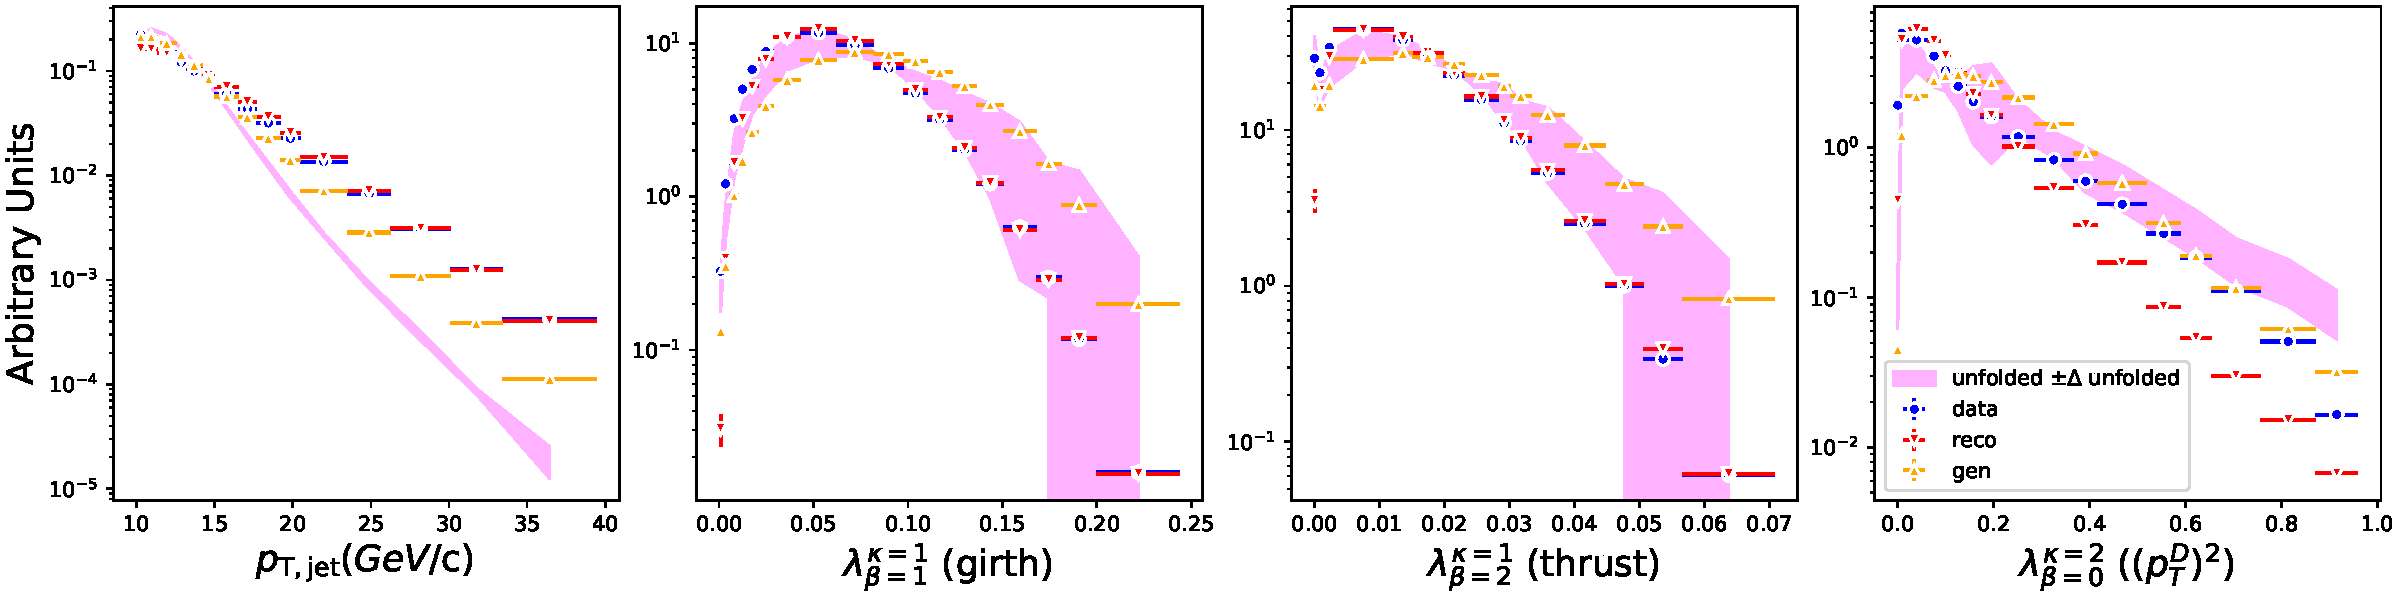
\includegraphics[width=\linewidth]{unfolded_hist/iteration_4.pdf}
%						\caption{Iteration 4}
%		\end{figure}
%	}
%	\only<3>{
%		\begin{figure}
%			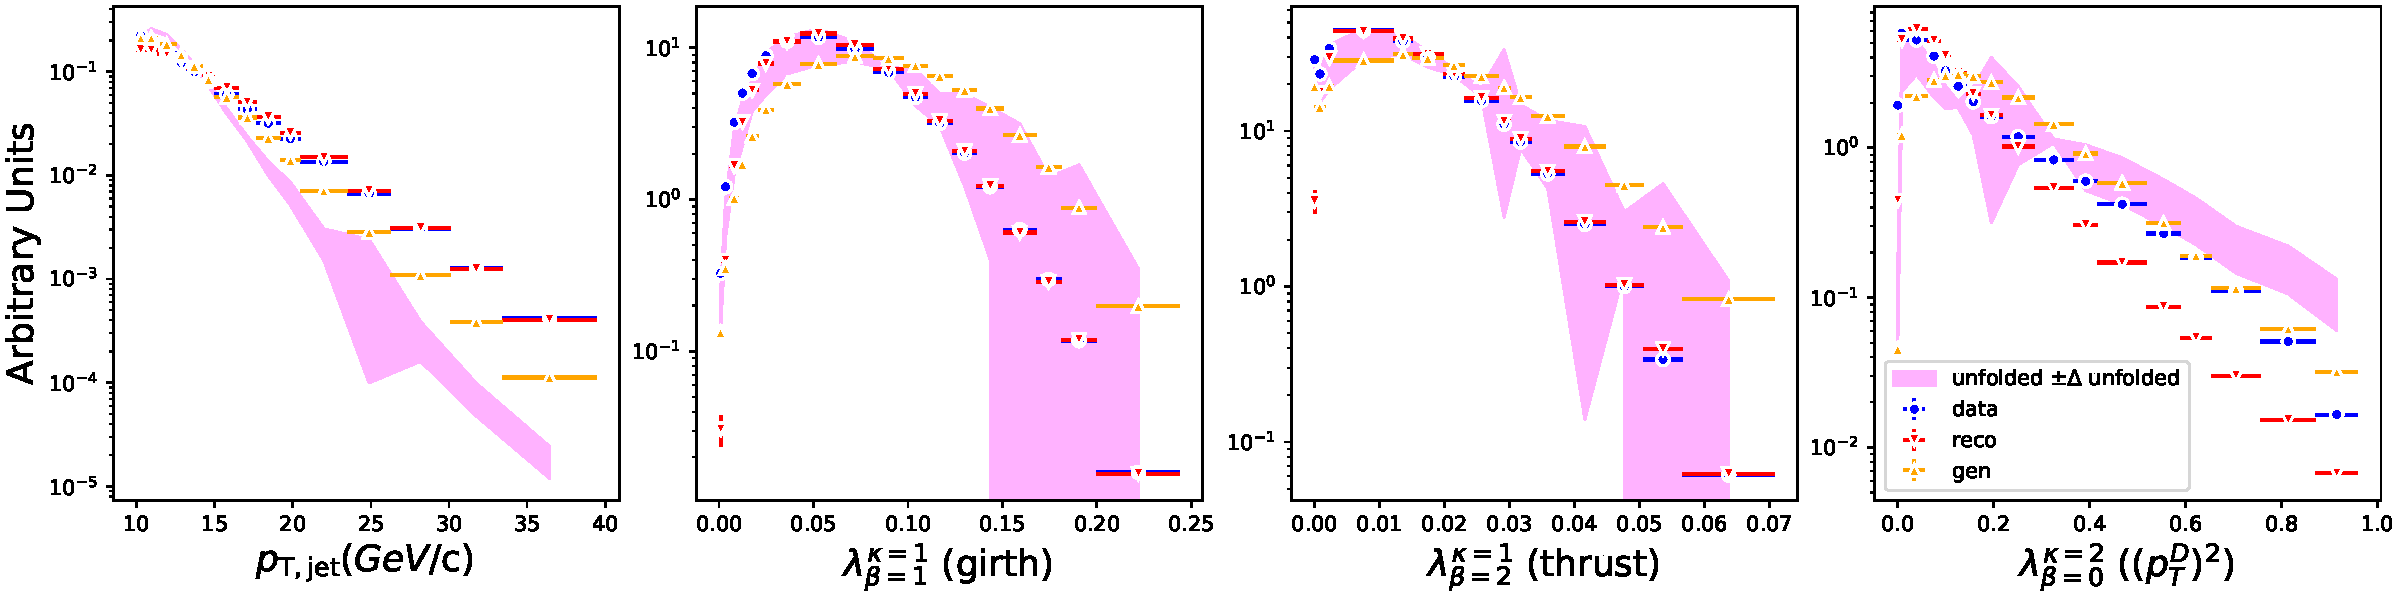
\includegraphics[width=\linewidth]{unfolded_hist/iteration_5.pdf}
%						\caption{Iteration 5}
%		\end{figure}
%	}
	\end{frame}
	
	\begin{frame}
		\frametitle{Conclusions and Outlook}
		\begin{itemize}
			\item Bootstraped ensembling results in better predictions which depend on phase space distribution of the features
			\item Omnifolded weights from bootstraped ensemble results in smoothing of sample-weights distributions
			\item  Unfolded distributions from bootstraped omnifold show uncertainties that increase with decrease in data statistics
			\item Need to run bigger ensembles to get better convergence of histograms with iterations
		\end{itemize}
	\end{frame}

\end{document}